\section{Introduction}
String theory is a framework that attempts to unify the two pillars of fundamental physics: quantum mechanics and general relativity.
It does so by replacing point-like particles with one-dimensional strings in the underlying mathematical description, so that the singular interaction vertices of point-particle Feynman diagrams give way to smooth two-dimensional worldsheets (Figure~\ref{fig:worldsheet}).
It is known to be consistent in 10 (for supersymmetric strings) and 26 (for bosonic strings) dimensions.
In the context of string theory, our 4-dimensional spacetime is then understood as the compactification of a higher-dimensional theory on an internal manifold.
Despite receiving no direct experimental validation, it remains an elegant framework of astonishing internal consistency.

\begin{figure}[ht]
\centering
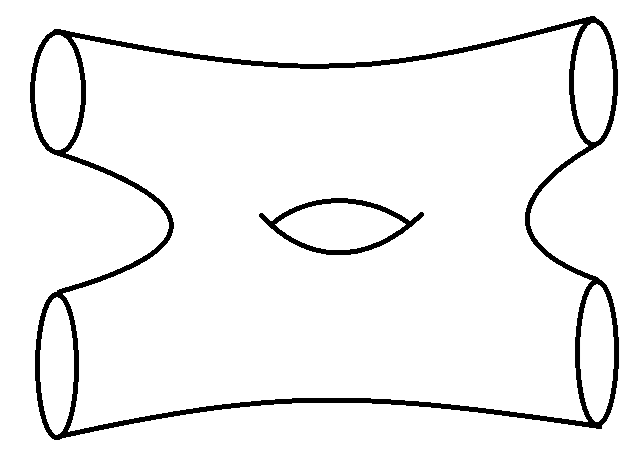
\includegraphics[width=0.5\textwidth]{worldsheet_amplitude.png}
\caption{A closed-string scattering amplitude is a smooth two-dimensional worldsheet. Where the Feynman diagrams of point particles meet at singular interaction vertices, string interactions are carried by the smooth topology of the worldsheet, with no distinguished interaction point.}
\label{fig:worldsheet}
\end{figure}

\[
\text{10d spacetime} = \underbrace{\mathbb{R}^{3,1}}_{\text{observed 4d}} \times \underbrace{M_6}_{\substack{\text{compact 6d} \\ \text{(curled up)}}}
\]

In 10 dimensions, there are five consistent superstring theories: type IIA, type IIB, heterotic SO(32), heterotic $E_8 \times E_8$, and type I.
These theories are related by various dualities, and are believed to be different limits of a single underlying theory, M-theory, in 11 dimensions (Figure~\ref{fig:duality-web}).
For instance, the type IIA and the heterotic $E_8 \times E_8$ theories are understood to arise from M-theory compactified on a circle and an interval, respectively.
The type IIB theory, in turn, arises as the decompactifying limit of the 9d theory obtained from M-theory on a torus.
The type I theory can be obtained from the type IIB theory by an orientifold projection (gauging worldsheet parity), and is related to the heterotic SO(32) theory by S-duality.

\begin{figure}[ht]
\centering
% PLACEHOLDER -- replace this tikzpicture with \includegraphics{figures/duality-web}
% once the artwork is supplied. Drawing brief: the web of five superstring theories with
% M-theory at the centre. Reductions of M-theory: on S^1 -> IIA, on the interval S^1/Z_2
% -> heterotic E_8 x E_8, on T^2 (decompactifying limit) -> IIB. Dualities: IIA <-> IIB
% (T), heterotic E_8 x E_8 <-> heterotic SO(32) (T), IIB <-> type I (orientifold Omega),
% type I <-> heterotic SO(32) (S).
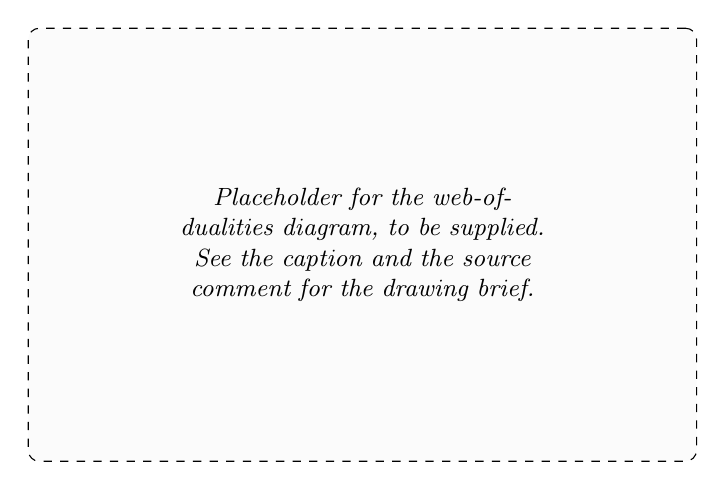
\begin{tikzpicture}
  \node[draw, dashed, rounded corners, fill=gray!3,
        minimum width=0.7\textwidth, minimum height=5.5cm,
        align=center, text width=0.62\textwidth, font=\small\itshape]
       {Placeholder for the web-of-dualities diagram, to be supplied.\\ See the caption and the source comment for the drawing brief.};
\end{tikzpicture}
\caption{The web of superstring dualities and their common origin in eleven-dimensional M-theory. Type IIA and heterotic $E_8\times E_8$ arise from M-theory on a circle ($S^1$) and on an interval ($S^1/\mathbb{Z}_2$). Type IIB arises as the decompactifying limit of M-theory on a two-torus ($T^2$), the nine-dimensional detour that this thesis seeks to bypass. Type I follows from a type IIB orientifold ($\Omega$) and is S-dual to heterotic SO(32), while the T-duality links relate the two type II and the two heterotic theories.}
\label{fig:duality-web}
\end{figure}

An intriguing feature of the type IIB theory is its conjectured \SLZ{} duality, which exchanges the fundamental string with the D1 brane.
This duality is believed to be an exact non-perturbative symmetry of the type IIB theory, and has received support from modular-invariant $R^4$ corrections to the effective action, as well as the existence of the (p, q) strings and 7-branes.
But why does the type IIB theory have such an \SLZ{} duality?
One may reconcile this with the M-theory origin of the type IIB theory, since \SLZ{} is the group of large diffeomorphisms of the torus, acting on its complex structure, which can be identified with the axio-dilaton.
Yet this explanation is unsatisfactory, as the \SLZ{} duality of the type IIB theory is a fundamental feature in 10d, and thus one should not have to take a detour through 9d to understand it.
This motivates seeking a higher-dimensional account in which the duality is manifest from the outset, without singling out a compactification circle: a 12d origin of the type IIB theory.

Indeed, after the construction of the 11d supergravity \cite{Nahm:1977tg,Cremmer1978}, it was soon realised that SO(10, 2) Majorana-Weyl spinors might offer a natural setting for a 12d supersymmetric theory of gravity \cite{Castellani:1982ke,Blencowe:1988sk}.
Later, through the study of the 6d (2,0) gravity theory \cite{Hull:1995xh,Witten:1995em}, the 7-brane backreacted vacua \cite{Vafa:1996xn}, and the Euclidean D(-1) instanton \cite{Tseytlin:1996it}, more evidence for an effective 12d interpretation of the type IIB theory has emerged.

However, the construction of a 10+2d supergravity \cite{Nishino:1997gq} has faced persistent conceptual obstructions, due to its non-compact little group and the lack of a momentum generator in its algebra \cite{Hewson:1997wv}.
To this day, no consistent 10+2d supergravity with 32 supercharges that reduces to the type IIB supergravity has been constructed. 
On the other hand, effective 12d perspectives, arising from branes \cite{Tseytlin:1996ne}, dualities \cite{Tseytlin:1996it}, and effective actions \cite{Minasian:2015bxa}, have proven more fruitful, providing concrete insights into the type IIB theory and its \SLZ{} duality.
These will be reviewed in this thesis.\footnote{
One may argue that the appearance of \SLZ{} is merely a manifestation of redundancy in the parameterisation we have chosen to describe the type IIB theory.
While it would be interesting to ask whether a formulation without this redundancy exists, and what it would imply for the other superstring theories and the web of dualities as a whole, that is not our focus here.
As long as no such formulation is known, the \SLZ{}-manifest description remains the one that reveals the web of dualities, and hence is the most natural one we have access to at the moment.
}

Beyond these formal motivations, a concrete new reason to revisit the question comes from holography, specifically the AdS/CFT correspondence.
It appears most concretely in the duality between M-theory and type IIA, where the near-horizon geometry of a stack of M2-branes, $\mathrm{AdS}_4 \times S^7/\mathbb{Z}_k$, is holographically dual to the ABJM theory \cite{Aharony:2008ug}.
The $\tfrac{1}{2}$-BPS circular Wilson loop of this theory admits a dual description as a wrapped M2-brane, whose action reproduces the Wilson-loop expectation value at large $N$ \cite{Giombi:2023vzu,Tseytlin:2024euk}.
The ABJM theory has no continuous coupling, but its discrete Chern-Simons level $k$ may be effectively treated as a coupling, and here it is geometrised as the size of the M-theory circle.
It is natural to ask whether an analogous relation holds on the type IIB side, between the $\mathrm{AdS}_5 \times S^5$ background and the $\mathcal{N}=4$ SYM theory, which carries its own \SLZ{} duality acting on its complexified coupling.
If the $\mathrm{AdS}_5 \times S^5$ background, like the D(-1) and D7 backgrounds, admits a 12d uplift, then wrapping a 12d object on a torus would geometrise the coupling of $\mathcal{N}=4$ SYM.
Addressing this question lies beyond the scope of this thesis, and would require a 12d interpretation of the D3 brane that sources the $\mathrm{AdS}_5 \times S^5$ background.
We therefore revisit the question of a 12d interpretation of the type IIB string theory, continuing this line of work, with additional motivation from the recent developments in AdS/CFT.

This review is motivated by two guiding questions: whether the type IIB theory has a higher-dimensional origin, and what the role and origin of its \SLZ{} duality are. These are pursued through the following concrete objectives:
\begin{enumerate}
    \item to establish a 12d interpretation of the type IIB axio-dilaton sector, by realising the D7 brane and D(-1) instanton backgrounds as a 12d Kaluza-Klein monopole and pp-wave, respectively, reduced on a torus, and to verify its consistency with supersymmetry (Section \ref{sec:axio-dilaton-12d}).
    \item to determine whether this interpretation extends beyond the axio-dilaton sector, by constructing a covariant 12d unification of the type IIB form fields (Section \ref{sec:covariant-unification}).
    \item to clarify the role of the D3 brane, whose worldvolume electromagnetic \SLZ{} duality is tied to the bulk \SLZ{} S-duality of the type IIB supergravity (Section \ref{sec:d3-self-duality}).
    \item to test the 12d interpretation with the higher-derivative corrections that appear to render \SLZ{} exact, and to clarify its limitations (Section \ref{sec:effective-actions}).
\end{enumerate}
We assess the extent to which each of these objectives is met in the concluding section.

This thesis is organised as follows. We first introduce the type IIB theory and discuss its puzzles.
For completeness, we review various attempts at formulating a 10+2d supergravity theory (Section~\ref{sec:12d-supergravity-attempts}).
We then turn to the 12d perspectives arising from branes and effective actions, beginning with the sector that most robustly admits a 12d interpretation, the axio-dilaton.
Here we show that the D7 background may be viewed as the 12d Kaluza-Klein monopole reduced on a torus, and the D(-1) background as a compactification of the 12d pp-wave.
Throughout, we present the analogous constructions on the type IIA side and discuss their consistency with supersymmetry.

We next discuss whether the higher-dimensional interpretation of the D(-1) instanton and the D7 brane backgrounds can be extended to other branes, and introduce a covariant 12d unification of the type IIB form fields.
In our proposal, the 12d uplift of the 5-form flux is a 12d 7-form flux, and the 10d self-duality condition on the 5-form is implemented as a 12d Hodge duality.

We then examine the D3 brane worldvolume action, noting that consistency requires the identification between the bulk \SLZ{} S-duality of type IIB supergravity and the \SLZ{} electromagnetic duality acting on the D3 brane worldvolume fields.
This interplay suggests that the D3 brane may play a special role in understanding 12d insights into the type IIB S-duality.

Lastly, we discuss how the higher-derivative corrections to the type IIB action may be interpreted from a 12d perspective, and demonstrate the limitations of such an interpretation.